\section{Using VST}

\subsection{The Trusted Base}

The soundness of our proof relies on a trusted base
, i.e. a foundation of specifications and implementations
that must stay correct with respect to the specifications.

\begin{itemize}
  \item \textbf{Calculus of Inductive Construction} : The intuitionistic logic
  used by Coq must be consistent in order to trust the proofs. We assumed that
  the functional extensionality was also consistent with that logic.

$
\begin{array}{c}
  \forall A\ B (f\ g : A \to B ),\\
  ( \forall x : A , f(x) = g(x) ) \implies f = g
\end{array}
$
  \item \textbf{CompCert} Clight model

  \item \textbf{\texttt{clightgen}} translation from \textbf{C} to
  \textbf{Clight}.
  VST does not support the verification of
  \texttt{o[i] = a[i] + b[i]}, the \texttt{forward} tactic will simply not work.
  This required us to rewrite the lines into:\\
  \texttt{aux1 = a[i];\\
  aux2 = b[i];\\
  o[i] = aux1 + aux2;}. This rewriting is done
  The trust of the proof relied on the trust of a correct translation from the
  initial version of \textit{TweetNaCl} to \textit{TweetNaclVerificable}.

  While this problem is still present, the Compcert developpers provided us with
  the \texttt{-normalize} option for \texttt{clightgen} which takes care of
  generating auxiliary variables in order to automatically derive these steps.
  The changes required for a C-code to make it Verifiable are now minimals.


  \item The \textbf{Coq kernel}, the \textbf{Ocaml compiler},
  the \textbf{Ocaml Runtime} and the \textbf{CPU}. These are common to all proofs
  done with this architecture \cite{2015-Appel,coq-faq}.
\end{itemize}

\subsection{Aliasing and Memory collision}

Necessity to go back into your specification multiple times to refine your model.
e.g. prove \texttt{M(o,a,b)} later notice that you can have aliasing, need to redefine
your theorem to prove \texttt{M(o,a,a)} (\textit{squaring}) and other variants such as:
\texttt{M(a,a,b)} and \texttt{M(b,a,b)}.

\begin{figure}[h]
  \begin{tikzpicture}
\draw (0,0) rectangle (3,0.3);
\draw[thick] (1,0) -- (1,0.3);
\draw[thick] (2,0) -- (2,0.3);
\node [anchor=east] (shn) at (0,0.15) {sh};
\node [anchor=north] (Moab) at (1.5,-0.5) {\texttt{M(o,a,b)}};
\draw[thick, -> ] (1.25, -0.6) -- (1.25, -0.5) -- (0.5,-0.1);
\draw[thick, -> ] (1.6, -0.6) -- (1.6, -0.5) -- (1.5,-0.1);
\draw[thick, -> ] (1.95, -0.6) -- (1.95, -0.5) -- (2.5,-0.1);

\node [anchor=north west, text width=6cm, align=left] (Sepoab) at (-0.5,-1.8)
  {\VSTess{sh [{ v_o $\!\!\}\!\!]\!\!\!$ <<(lg16)-- o}\\[-0.2em]
  \VSTess{sh [{ v_a $\!\!\}\!\!]\!\!\!$ <<(lg16)-- a}\\[-0.2em]
  \VSTess{sh [{ v_b $\!\!\}\!\!]\!\!\!$ <<(lg16)-- b}};


\begin{scope}[yshift=0 cm,xshift=4.5 cm]
  \draw (0,0) rectangle (2,0.3);
  \draw[thick] (1,0) -- (1,0.3);
  % \draw[thick] (2,0) -- (2,0.3);
  \node [anchor=east] (shm) at (0,0.15) {sh};
  \node [anchor=north] (Mcaa) at (1,-0.5) {\texttt{M(c,c,a)}};
  \draw[thick, -> ] (0.75, -0.6) -- (0.75, -0.5) -- (0.4,-0.1);
  \draw[thick, -> ] (1.1, -0.6) -- (1.1, -0.5) -- (0.6,-0.1);
  \draw[thick, -> ] (1.45, -0.6) -- (1.45, -0.5) -- (1.5,-0.1);

  \node [anchor=north west, text width=6cm, align=left] (Sepoab) at (-0.5,-1.8)
    {\VSTess{sh [{ v_c $\!\!\}\!\!]\!\!\!$ <<(lg16)-- c}\\[-0.2em]
    \VSTess{sh [{ v_a $\!\!\}\!\!]\!\!\!$ <<(lg16)-- a}};
\end{scope}

\draw[dashed] (-0.5,-1.2) -- +(8,0);
\node [anchor=north west] (sep) at (-0.5,-1.2) {In Separation Logic:};

\begin{scope}[yshift=-4.25 cm,xshift=2 cm]
  \draw (0,0) rectangle (2,0.3);
  \draw[thick] (1,0) -- (1,0.3);
  \node [anchor=east] (shm) at (0,0.15) {sh\;};

  \draw (0,0.5) rectangle (1,0.8);
  \node [anchor=east] (shm) at (0,0.65) {Ews};

  \draw[thick] (2,0) -- (2,0.3);
  \node [anchor=north west] (Mcaa) at (0.15,-0.5) {\texttt{M(a,c,\_121665)}};
  \draw[thick, -> ] (0.75, -0.6) -- (0.75, -0.5) -- (0.5,-0.1);
  \draw[thick, -> ] (1.1, -0.6) -- (1.1, -0.5) -- (1.5,-0.1);
  \draw[thick, -> ] (2.0, -0.6) -- (2.45, -0.2) -- (2.45, 0.3) -- (2.2, 0.65) -- (1.5,0.65);

  \node [anchor=north west, text width=6cm, align=left] (Sepoab) at (-0.5,-1.8)
    {\VSTess{sh [{ v_a $\!\!\}\!\!]\!\!\!$ <<(lg16)-- a}\\[-0.2em]
    \VSTess{sh [{ v_c $\!\!\}\!\!]\!\!\!$ <<(lg16)-- c}\\[-0.2em]
    \VSTess{Ews [{ __121665 $\!\!\}\!\!]\!\!\!$ <<(lg16)-- _121665}
    };
\end{scope}
\draw[dashed] (0.5,-5.45) -- +(6,0);
\node [anchor=north west] (sep) at (0.5,-5.45) {In Separation Logic:};
\end{tikzpicture}%

  \caption{Aliasing and Separation Logic}
  \label{tk:MemSame}
\end{figure}

Prove \texttt{M(o,a,b)} where o is a \texttt{list $\Z$} and then realize that
\texttt{o} can be a list of \textit{undefined} (\texttt{list val}). Thus needs
to reprove the above theorem again.

% \begin{figure}[h]
%   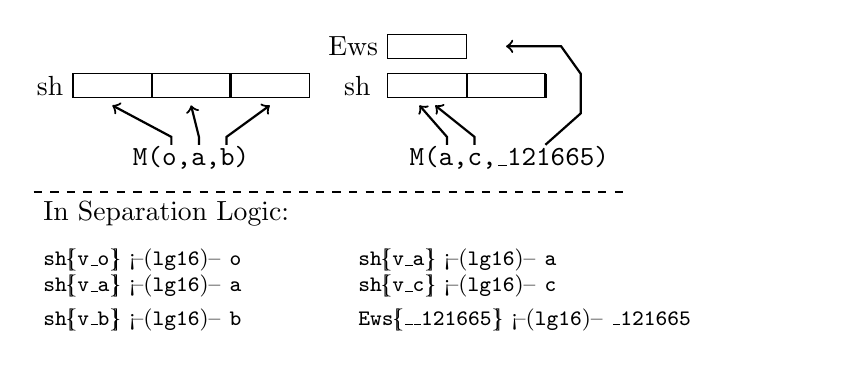
\begin{tikzpicture}
\def\-{\raisebox{.75pt}{-}}

\draw (0,0) rectangle (3,0.3);
\draw[thick] (1,0) -- (1,0.3);
\draw[thick] (2,0) -- (2,0.3);
\node [anchor=east] (shn) at (0,0.15) {sh};
\node [anchor=north] (Moab) at (1.5,-0.5) {\texttt{M(o,a,b)}};
\draw[thick, -> ] (1.25, -0.6) -- (1.25, -0.5) -- (0.5,-0.1);
\draw[thick, -> ] (1.6, -0.6) -- (1.6, -0.5) -- (1.5,-0.1);
\draw[thick, -> ] (1.95, -0.6) -- (1.95, -0.5) -- (2.5,-0.1);

\node [anchor=north west, text width=6cm, align=left] (Sepoab) at (-0.5,-1.8)
  {\footnotesize{$\mathtt{sh [\!\!\{ v\_o \}\!\!]\ \textrm{<\!--(}lg16\textrm{)--}\ o}$\\
  $\mathtt{sh [\!\!\{ v\_a \}\!\!]\ \textrm{<\!--(}lg16\textrm{)--}\ a}$\\
  $\mathtt{sh [\!\!\{ v\_b \}\!\!]\ \textrm{<\!--(}lg16\textrm{)--}\ b}$}};


\begin{scope}[yshift=0 cm,xshift=4 cm]
  \draw (0,0) rectangle (2,0.3);
  \draw[thick] (1,0) -- (1,0.3);
  \node [anchor=east] (shm) at (0,0.15) {sh\;};

  \draw (0,0.5) rectangle (1,0.8);
  \node [anchor=east] (shm) at (0,0.65) {Ews};

  \draw[thick] (2,0) -- (2,0.3);
  \node [anchor=north west] (Mcaa) at (0.15,-0.5) {\texttt{M(a,c,\_121665)}};
  \draw[thick, -> ] (0.75, -0.6) -- (0.75, -0.5) -- (0.4,-0.1);
  \draw[thick, -> ] (1.1, -0.6) -- (1.1, -0.5) -- (0.6,-0.1);
  \draw[thick, -> ] (2.0, -0.6) -- (2.45, -0.2) -- (2.45, 0.3) -- (2.2, 0.65) -- (1.5,0.65);

  \node [anchor=north west, text width=6cm, align=left] (Sepoab) at (-0.5,-1.8)
    {\footnotesize{$\mathtt{sh [\!\!\{ v\_a \}\!\!]\ \textrm{<\!--(}lg16\textrm{)--}\ a}$\\
    $\mathtt{sh [\!\!\{ v\_c \}\!\!]\ \textrm{<\!--(}lg16\textrm{)--}\ c}$\\
    $\mathtt{Ews} \mathtt{[\!\!\{ \_\_121665 \}\!\!]\ \textrm{<\!--(}lg16\textrm{)--}\ \_121665}$}};

\end{scope}

\draw[dashed] (-0.5,-1.2) -- +(7.5,0);
\node [anchor=north west] (sep) at (-0.5,-1.2) {In Separation Logic:};

\end{tikzpicture}

%   \caption{Memory Share and Separation Logic}
%   \label{tk:MemSame}
% \end{figure}

\subsection{How to be efficient with VST?}

This approach is \textbf{slow}, \textbf{tedious} and \textbf{frustrating}.
The time cost way to big for such a proof and definitively not applicable for a
cryptographic engineer.

Necessity to prove everything at least 3 to 4 times (high level, low level, C-link).

The \texttt{forward} and \texttt{entailer} tactics are slow.

Specification and proofs does not need to be in the same file (as initially \textit{implied}
by the examples provided by the VST repository). Putting the specification of each
functions in separate file reduce the amount of dependencies. One does not need
to wait for the proof of correctness of \texttt{M(o,a,b)} to compile the proof of \texttt{crypto\_scalarmult(q,n,p)}.
This separation allows a high degree of parallelism during compilation \texttt{make -j},
greatly reducing the amount of time required.

Three years ago:
\url{https://www.imperialviolet.org/2014/09/11/moveprovers.html}
\url{https://www.imperialviolet.org/2014/09/07/provers.html}

\subsection{Pointers arithmetic, arrays and types}


It is to be noted that the \texttt{clightgen} tool has not been formally verified.

\texttt{clightgen -normalize}

% Not true since VST 2.0
%
% Assuming that \texttt{b} is of type \texttt{long long}, the following expression
% will not be type-checked by VST.
%
% \texttt{b = 1 - b;}
%
% \texttt{1} is interpreted by cligthgen as \texttt{Vint} (\textit{Value of int})
% while \texttt{b} is interpreted as \texttt{Vlong} (\textit{Value of long}),
% resulting in an error. To solve this, we need to prefix \texttt{1} by an
% explicit cast in C into the correct type. As a result, any constants used in this
% implementation had to be casted to the correct type
% (in \textit{TweetNaclVerificable}) to pass typecheck.

\subsection{Verifiying for loops: head and tail recursion}

While the final state of a For loops can be computed by a simple recursive function,
we must define invariants that are true for each step of the iteration.

\begin{coqD}
Variable T : Type.
Variable g : nat -> T -> T.

Fixpoint rec_fn (n:nat) (s:T) :=
  match n with
  | 0 => s
  | S n => (rec_fn n (g n s))
  end.

Fixpoint rec_fn_rev_acc (n:nat) (m:nat) (s:T) :=
  match n with
  | 0 => s
  | S n => g (m - n - 1) (rec_fn_rev_acc n m s)
  end.

Definition rec_fn_rev (n:nat) (s:T) :=
  rec_fn_rev_acc n n s.

Lemma Tail_Head_equiv :
  forall (n:nat) (s:T),
  rec_fn n s = rec_fn_rev n s.
\end{coqD}


In order to prove the for loops, we must define invariants.
Those have to be


TODO:
How many lines of specification ?
How many lines of proofs ?
How long did it take ?
